% !TeX spellcheck = en_GB
\documentclass[main.tex]{subfiles}

\begin{document}
\chapter{Results}
\lhead{Results}
\label{chap:results}

\section{English LUKE Reproduction}%
\label{sec:English LUKE Reproduction}
\begin{table}[H]
	\begin{center}
		\begin{tabular}{l c c c c c}
			Model & Micro avg. & LOC & PER & ORG & MISC \\
			\hline
			LUKE large & $94.00 \pm  0.2$ & $94.99 \pm  0.1$ & $97.19 \pm  0.1$ & $93.63 \pm  0.3$ & $85.29 \pm  1.0$ \\
			LUKE base & $93.42 \pm  0.2$ & $94.67 \pm  0.2$ & $96.89 \pm  0.2$ & $92.41 \pm  0.2$ & $84.94 \pm  0.7$
		\end{tabular}
	\end{center}
	\caption{Mean F1\pro\ scores and standard deviation over five repetitions of fine-tuning and evaluating LUKE on CoNLL-2003 for each model size.}
	\label{tab:lukeF1s}
\end{table}
Yamada et al. report micro avg. F1 scores of 94.3\pro\ and 93.3\pro\ for LUKE large and base, respectively \cite{yamada2020luke}.
In both cases, this is within two standard deviations of our fine-tuning results.
This is expected and we conclude that the reproduction was successful.
However, the variability of fine-tuning is also highlighted here and will be discussed in Section~\ref{sec:fine-tuning-exp}.
% However, it also highlights the variability of the fine-tuning.
% With margins between top-performing models being as small as they are \cite{pwc21ner}, whoever can claim SOTA may well come down to who got the luckiest seeds.
% This could be mitigated by reporting the mean of several fine-tunings, but Yamada et al. at least do not mention having done multiple fine-tunings.

\section{Pretraining of DaLUKE}
\label{sec:Pretraining of DaLUKE}

\begin{table}[H]
    \centering
    \begin{tabular}{l|rrrrrr}
        Top $k$ accuracy [\pro] & $k=1$  & $k=3$ & $k=5$ & $k=10$ & $k=25$ & $k=50$\\\hline
        Masked words            & 24.82       & 31.54      & 34.96      & 40.27       & 48.15       & 54.02      \\
        Masked entities         & 56.17       & 68.58      & 73.58      & 79.78       & 86.36       & 90.27
    \end{tabular}
    \caption{
        The main pretrained model performance in the last of 150 epochs.
        The measures are frequency of correct prediction on the two mask prediction tasks, when considering a prediction to be correct if the true token is one $k$ most likely labels according to the model softmax output.
    }
    \label{tab:mainpre}
\end{table}\noindent

\begin{figure}[H]
    \centering
    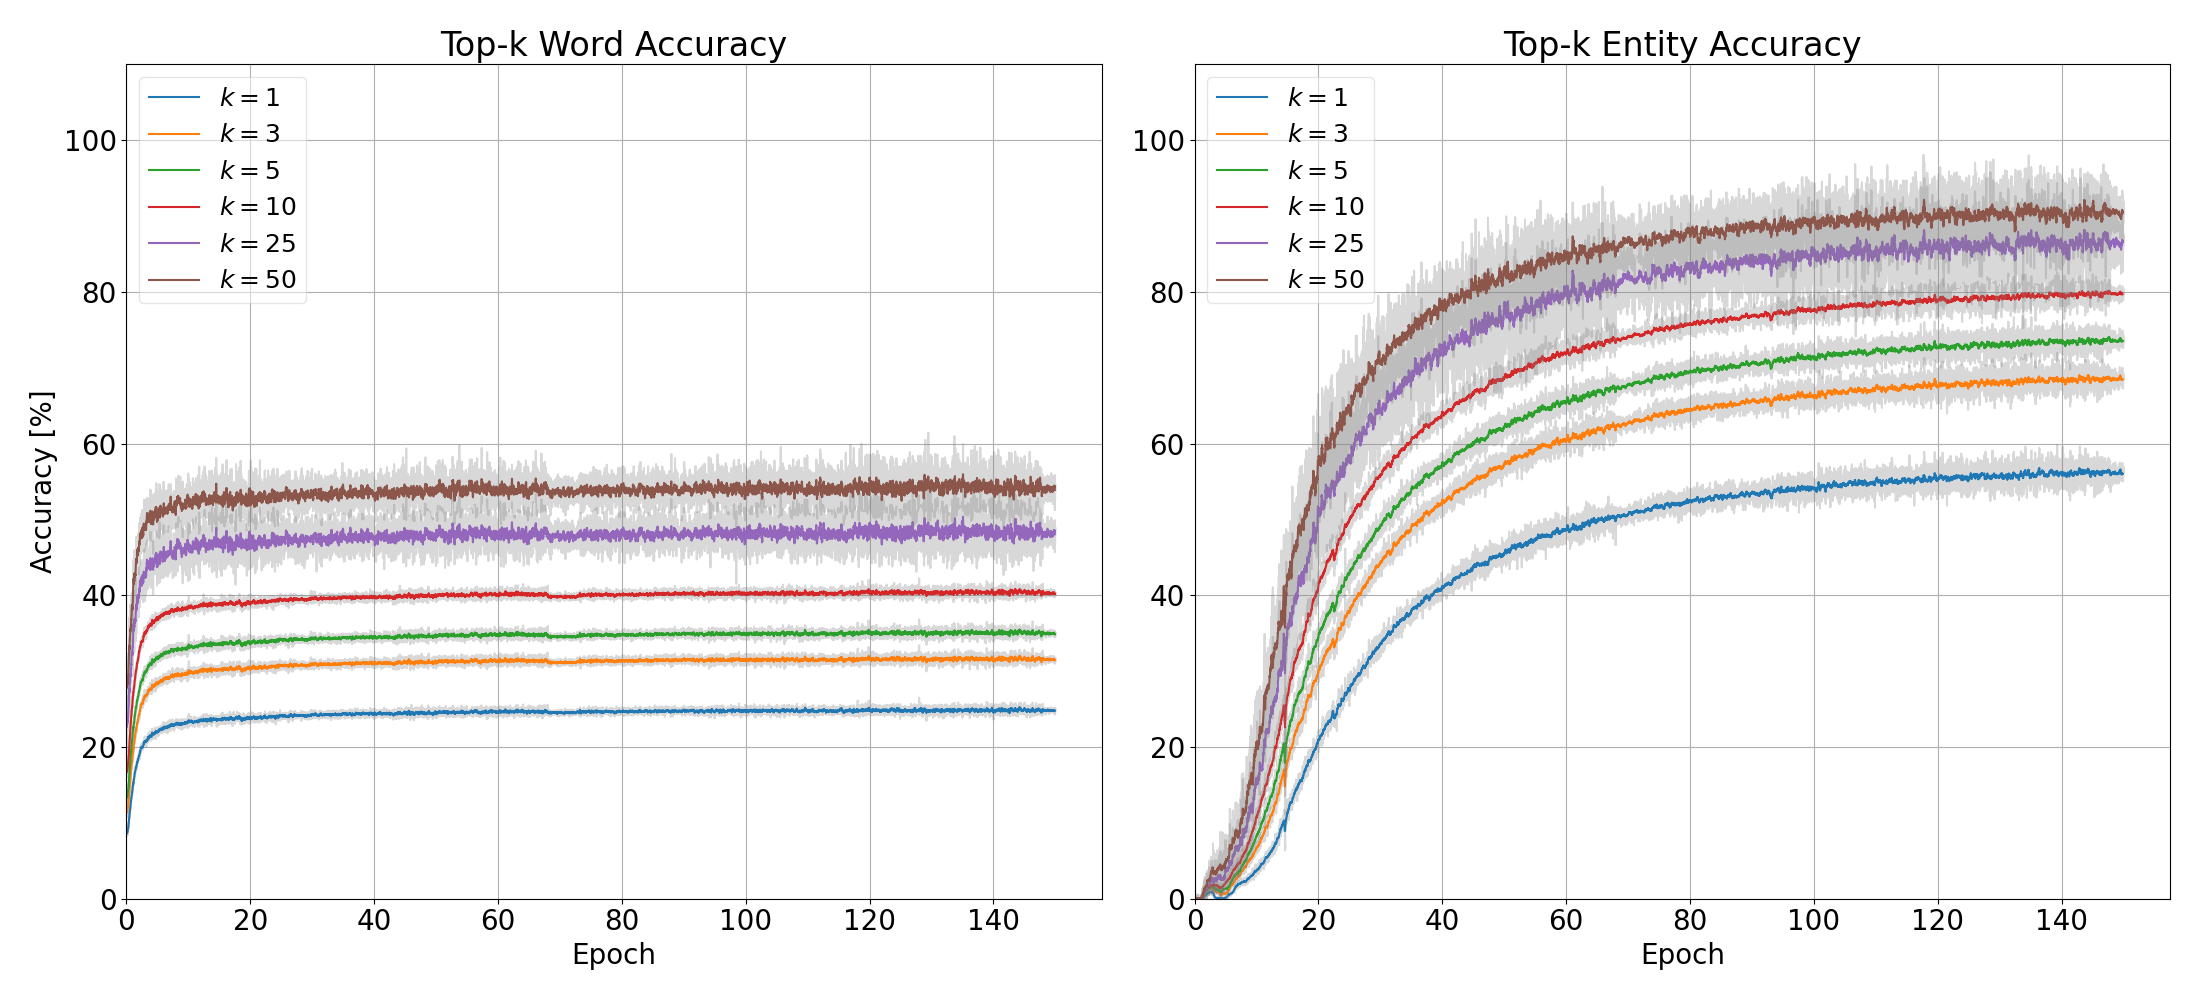
\includegraphics[width=\textwidth]{pretrain-acc}
    \caption{Masked subwords and masked entity accuracy throughout pretraining.
    The curves are smoothed with a rolling average.}
    \label{fig:pretrain-acc}
\end{figure}\noindent

\begin{figure}[H]
    \centering
    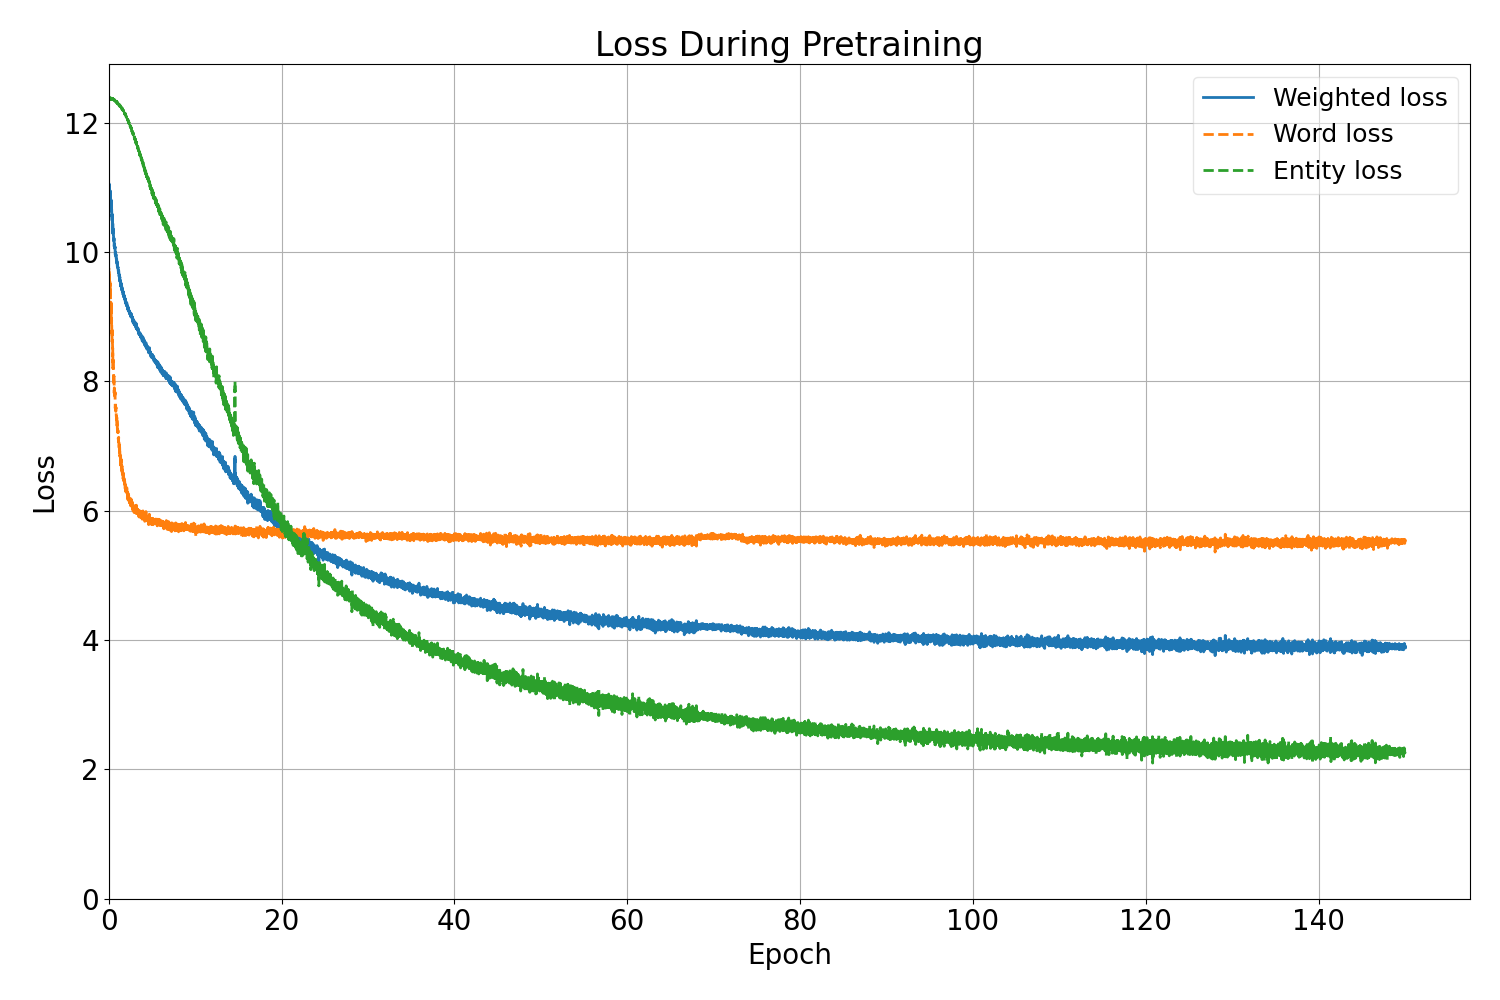
\includegraphics[width=.7\textwidth]{loss}
    \caption{Loss throughout pretraining for both pretraining tasks as well as total (weighted) loss, which is the average of the two.}
    \label{fig:loss}
\end{figure}\noindent
The masked subwords and masked entity accuracies are shown on Figure \ref{fig:pretrain-acc}.
The former converges quickly, achieving close to top accuracy in less than a tenth of the full training time, while the latter keeps improving throughout the training.
That the masked language modeling performance from BERT is quickly maximized is, however, perhaps not surprising, as many of the relevant weights are initialized from an already trained model which has been pretrained on the exact same task.
The loss shown on Figure \ref{fig:loss} mirrors the accuracy with masked subword loss converging quickly, after which falling entity loss becomes the driving factor behind the falling total loss.

\section{Danish Named Entity Recognition}%
\label{sec:nerres}

\subsection{Main Benchmark: Our Results and Reproduction}
\begin{enumerate}
    \item Inkludér træningskurve for NER
\end{enumerate}

              % precision    recall  f1-score   support

 % ┆   ┆   LOC     0.8365    0.9062    0.8700        96
 % ┆   ┆  MISC     0.7652    0.7273    0.7458       121
 % ┆   ┆   ORG     0.7956    0.6770    0.7315       161
 % ┆   ┆   PER     0.9441    0.9389    0.9415       180

 % ┆ micro avg     0.8467    0.8118    0.8289       558
 % ┆ macro avg     0.8354    0.8124    0.8222       558
% weighted avg     0.8440    0.8118    0.8262       558

              % precision    recall  f1-score   support

 % ┆   ┆   LOC     0.8365    0.9062    0.8700        96
 % ┆   ┆   ORG     0.7956    0.6770    0.7315       161
 % ┆   ┆   PER     0.9441    0.9389    0.9415       180

 % ┆ micro avg     0.8690    0.8352    0.8518       437
 % ┆ macro avg     0.8588    0.8407    0.8477       437
% weighted avg     0.8658    0.8352    0.8484       437
\begin{table}[H]
        \footnotesize
        \begin{center}
                \begin{tabular}{l l | c c c c | c c c c}
                    \multirow{2}{*}{Model name} & \multirow{2}{*}{Trained on} & \multicolumn{4}{c|}{Micro Avg. [\pro]} & \multicolumn{4}{c}{Class F1 [\pro]}\\
                                      &           & F1             & Prec.          & Rec.           & F1 {\tiny\textdiscount MISC} & LOC            & PER            & ORG            & MISC \\\hline
                        DaLUKE        & DaNE      & 82.89          & 84.67          & 81.18          & 85.18                        & \textbf{87.00} & \textbf{94.15} & 73.15          & 74.58 \\\hline
                        DaNLP da-BERT & DaNE      & --             & --             & --             & 84.04                        & 83.90          & 92.82          & 72.98          & -- \\
                        NERDA m-BERT  & DaNE      & 79.22          & 82.12          & 76.52          & 81.71                        & 83.50          & 92.61          & 66.90          & 70.34 \\
                        NERDA Ælæctra & DaNE      & 70.58          & 76.14          & 65.77          & 74.54                        & 77.32          & 86.93          & 56.18          & 56.39 \\
                        DaCy medium   & DaNE      & 78.32          & 78.32          & 78.32          & 80.50                        & 83.96          & 90.41          & 66.23          & 70.09 \\
                        DaCy large    & DaNE      & \textbf{84.91} & \textbf{86.16} & \textbf{83.69} & \textbf{86.89}               & 85.29          & \textbf{94.15} & \textbf{79.04} & \textbf{78.05} \\
                        DaNLP spaCy   & DaNE      & 73.75          & 76.15          & 71.51          & 75.73                        & 75.96          & 87.87          & 59.57          & 66.06 \\
                        DaNLP Flair   & DaNE      & --             & --             & --             & 81.78                        & 84.82          & 93.15          & 62.95          & -- \\
                        Polyglot      & Wikipedia & --             & --             & --             & 64.18                        & 64.95          & 78.74          & 39.30          & -- \\
                        daner         & ITU CDT   & --             & --             & --             & 56.52                        & 59.49          & 70.40          & 28.29          & -- \\
                \end{tabular}
        \end{center}
        \caption{F1\pro-scores of Danish NER models of the DaNE testing dataset consisting of 565 sentences.}
        \label{tab:DaNE}
\end{table}\noindent
DaLUKE fails to achieve SOTA on DaNE, being beaten only by DaCy large.
However, it does beat da-BERT on which it is based, indicating that the extra pretraining and entity understanding indeed has added some value to the model.
Interestingly, DaLUKE still manages to pull off a first place in the LOC category and ties DaCy large in PER, while falling behind in both ORG and MISC.
One possible reason may be the pretraining dataset.
Excluding the transferred da-BERT weights, it is pretrained solely on Wikipedia unlike DaCy.
While we have not investigated it further, it is possible that there are more articles on locations and people than there are on organizations and miscellaneous entities.

Ultimately, DaLUKE still performs at a high level and shows its promise for entity modeling.

\subsection{Additional Datasets}
              % precision    recall  f1-score   support

 % ┆   ┆   LOC     0.8298    0.8041    0.8168        97
 % ┆   ┆  MISC     0.0849    0.3000    0.1324        30
 % ┆   ┆   ORG     0.4710    0.6915    0.5603        94
 % ┆   ┆   PER     0.8994    0.9527    0.9253       169

 % ┆ micro avg     0.6054    0.8026    0.6902       390
 % ┆ macro avg     0.5713    0.6871    0.6087       390
% weighted avg     0.7162    0.8026    0.7493       390
              % precision    recall  f1-score   support

 % ┆   ┆   LOC     0.8298    0.8041    0.8168        97
 % ┆   ┆   ORG     0.4710    0.6915    0.5603        94
 % ┆   ┆   PER     0.8994    0.9527    0.9253       169

 % ┆ micro avg     0.7397    0.8444    0.7886       360
 % ┆ macro avg     0.7334    0.8161    0.7675       360
% weighted avg     0.7688    0.8444    0.8008       360
\begin{table}[H]
        \footnotesize
        \begin{center}
                \begin{tabular}{l l | c c c c | c c c c}
                    \multirow{2}{*}{Model name} & \multirow{2}{*}{Trained on} & \multicolumn{4}{c|}{Micro Avg. [\pro]} & \multicolumn{4}{c}{Class F1 [\pro]}\\
                                      &                & F1             & Prec.          & Rec.           & F1 {\tiny\textdiscount MISC} & LOC & PER & ORG & MISC \\\hline
                    DaLUKE        & DaNE           & \textbf{69.02} & \textbf{60.54}          & 80.26          & 78.86                        & \textbf{81.68} & \textbf{92.53} & 56.03 & 13.24 \\\hline
                        DaNLP da-BERT & DaNE           & --             & & & \textbf{79.23}               & 78.64 & 93.45 & \textbf{56.88} & -- \\
                        NERDA m-BERT  & DaNE           & 66.37          & 58.08          & 77.44          & 76.60                        & 76.33 & 92.08 & 52.53 & 12.41 \\
                        NERDA Ælæctra & DaNE           & 66.28          & 59.96          & 74.10          & 76.09                        & 74.87 & 90.32 & 53.00 & 13.24 \\
                        DaCy medium   & DaNE           & 65.61          & 55.73          & 79.74          & 75.03                        & 76.06 & 92.09 & 48.74 & 12.59 \\
                        DaCy large    & DaNE           & 68.45          & 58.86          & \textbf{81.79} & 79.02                        & 79.02 & \textbf{92.53} & 58.04 & \textbf{15.48} \\
                        DaNLP spaCy   & DaNE           & 64.11          & 55.92          & 75.13          & 72.70                        & 72.73 & 88.33 & 46.51 & 12.31 \\
                        DaNLP Flair   & DaNE           & --             & --             & --             & 76.16                        & 80.21 & 94.35 & 36.96 & -- \\
                        Polyglot      & Wikipedia      & --             & --             & --             & 64.10                        & 69.74 & 78.38 & 24.69 & -- \\
                        daner         & ITU CDT        & --             & --             & --             & 59.89                        & 58.16 & 73.63 & 26.09 & -- \\
                \end{tabular}
        \end{center}
        \caption{F1\pro\ scores of Danish NER models of the Plank test set consisting of 565 sentences.}
        \label{tab:Plank}
\end{table}

              % precision    recall  f1-score   support

 % ┆   ┆   LOC     0.7626    0.7085    0.7346      5242
 % ┆   ┆   ORG     0.6497    0.3347    0.4418      4078
 % ┆   ┆   PER     0.7239    0.7757    0.7489      4378

 % ┆ micro avg     0.7267    0.6187    0.6684     13698
 % ┆ macro avg     0.7121    0.6063    0.6418     13698
% weighted avg     0.7166    0.6187    0.6520     13698
\begin{table}[H]
        \footnotesize
        \begin{center}
                \begin{tabular}{l l | c c c | c c c }
                    \multirow{2}{*}{Model name} & \multirow{2}{*}{Trained on} & \multicolumn{3}{c|}{Micro Avg. [\pro]} & \multicolumn{3}{c}{Class F1 [\pro]}\\
                        & & F1 & Prec. & Rec. & LOC & PER & ORG \\
                        \hline
                    DaLUKE & DaNE & \textbf{66.84} & \textbf{72.67} & 61.87 & 73.46 & 74.89 & 44.18 \\\hline
                        DaNLP da-BERT & DaNE & 65.66 & 68.37 & 63.16 & 72.08 & 74.49 & 40.05 \\
                        NERDA m-BERT & DaNE & 63.40 & 61.28 & 65.68 & 70.72 & 76.87 & 48.35 \\
                        NERDA Ælæctra & DaNE & 48.65 & 48.32 & 48.99 & 56.63 & 69.89 & 24.02 \\
                        DaCy medium & DaNE & 60.05 & 58.37 & 61.84 & 70.71 & 73.74 & 39.27 \\
                        DaCy large & DaNE & 64.55 & 62.18 & \textbf{67.11} & \textbf{74.11} & \textbf{77.18} & \textbf{49.78} \\
                        DaNLP spaCy & DaNE & 59.55 & 58.52 & 60.61 & 68.68 & 71.63 & 38.76 \\
                        DaNLP Flair & DaNE & 65.04 & 70.74 & 60.19 & 70.08 & 74.36 & 43.67 \\
                        Polyglot & Wikipedia & 61.99 & 66.34 & 58.18 & 72.45 & 69.15 & 35.33 \\
                        daner & ITU CDT & 46.59 & 51.54 & 42.51 & 56.15 & 54.51 & 14.76 \\
                \end{tabular}
        \end{center}
        \caption{F1\pro\ scores of Danish NER models of the WikiANN test set consisting of 10,000 sentences.}
        \label{tab:WikiANN}
\end{table}
When fine-tuned on DaNE, DaLUKE achieves achieves SOTA both when evaluated on the Plank and WikiANN test sets, though only by a small margin on Plank.
This is unexpected given that DaLUKE is beaten on the DaNE test set.
It may indicate a better generalization ability, which, if true, is indeed a desirable property.
However, less exciting reasons for this behaviour may well be more likely.
With Plank, the difference is miniscule and may simply be explained by variance.
As shown in Section \ref{sec:English LUKE Reproduction} and \ref{sec:luke-stability}, this affects LUKE on CoNLL-2003 and DaLUKE on DaNE.
The performance discrepancy on WikiANN may be even less exciting:
That DaLUKE is pretrained directly on similar, annotated Wikipedia data, violating the principle that the training and test sets should be disjoint.

\end{document}
